\def\difficulty{2}
\sujet{Hough transform and line detection}
\index{Segmentation!Hough Transform}

\begin{note}This tutorial introduces the Hough transform. Line detection operators are implemented.\end{note}
\vspace*{-8pt}
\section{Introduction}\vspace*{-8pt}
This tutorial deals with line detection in an image. For a given point of coordinates $(x,y)$ in $\R^2$, there exists an infinite number of lines going by this point, with different angles $\theta$. These lines are represented by the following equation:
$$\rho=x\cdot\cos (\theta) + y\cdot\sin (\theta).$$

Thus, for each point $(x,y)$ (Fig. \ref{fig:points}) corresponds a curve parametered by $[\theta, \rho]$, where $\theta\!\in\![0;\!2\pi]$ (Fig. \ref{fig:hough}). The intersection of these curves represents a line (in this case, $y=x$).

\vspace*{-8pt}

\begin{figure}[htbp]
 \centering\caption{Representation of the Hough transform.}
 \subfloat[Different points in $\R^2$.]{
\resizebox{.35\textwidth}{!}{
 \begin{tikzpicture}[domain=0:4]

% axis
    \draw[->] (-0.2,0) -- (4.2,0) node[right] {$X$};
    \draw[->] (0,-1.2) -- (0,4.2) node[above] {$Y$};
	 
	 % points
	 \foreach \Point in {(1,1), (2,2), (3,3)}{
			\node[color=blue] at \Point {\textbullet};
			\node[color=blue] at \Point [above]{\Point};
	 }
	 
    \draw[color=red] plot[id=x] (\x,{\x}) node[right] {$y=x$};

	\label{fig:points}
\end{tikzpicture}}
 } \hspace{1.5cm}
\subfloat[Hough transform of the 3 points.]{\resizebox{.35\textwidth}{!}{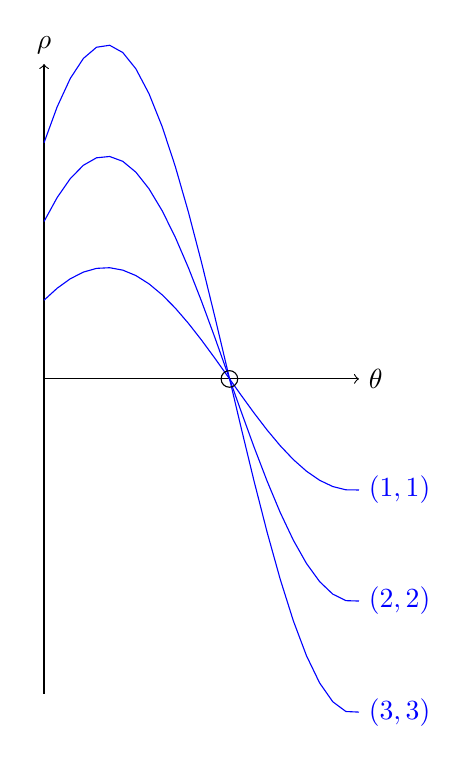
\begin{tikzpicture}[domain=0:4]
    \draw[->] (0,0) -- (4,0) node[right] {$\theta$};
    \draw[->] (0,-4) -- (0,4) node[above] {$\rho$};
	 \draw[domain=0:4,color=blue] plot (\x, {cos(\x r)+sin(\x r)}) node[right] {$(1,1)$};
	 \draw[domain=0:4,color=blue] plot (\x,{2*cos(\x r)+2*sin(\x r)}) node[right] {$(2,2)$};
	 \draw[domain=0:4,color=blue] plot (\x, {3*cos(\x r)+3*sin(\x r)}) node[right] {$(3,3)$};
	 \draw (2.354,0) circle[radius=3pt];
\end{tikzpicture}}
\label{fig:hough}
}\vspace*{-10pt}
\end{figure}

\vspace*{-10pt}

\section{Algorithm}
The (general and simple) method for line detection is then:
\begin{enumerate}
 \item Compute contours detections (get a binary image BW).
 \item Apply the Hough transform on the contours BW.
 \item Detect the maxima of the Hough transform.
 \item Get back in the Euclidean space and draw the lines on the image.
\end{enumerate}
Results should look like in Fig. \ref{fig:tutorial:hough:results}.

\begin{figure}[htbp]
 \centering\caption{Lines detection via Hough transform.}
 \subfloat[Hough transform and maxima detection. Angles $\theta$ are represented in abscissa, pixels $\rho$ are represented in ordinates. The detection of the absolute maxima of this images will lead to the lines.]{\includegraphics[width=.55\textwidth]{hough.png}}
 \hfill
 \raisebox{2.25\baselineskip}{\subfloat[Line detection.]{\hspace*{-5pt}{\includegraphics[width=.5\textwidth,angle=90]{detectionT.png}}}}\hspace*{-2pt}\null
 \label{fig:tutorial:hough:results}
\end{figure}


\section{Hough transform}
\begin{qbox}
Code a function that will transform each point of a binary image into a curve in the Hough space. For each curve, increment each pixel by one in the Hough space.
\end{qbox}

\section{Maxima detection}
\begin{qbox}
Use or code a function to detect maxima (regional maxima). For each maximum, keep only one point.
\end{qbox}

\section{Display lines}
\begin{qbox}
For each maximum, display the corresponding line above the original image.
\end{qbox}
